\documentclass{article} % For LaTeX2e
\usepackage{nips13submit_e,times}
\usepackage{hyperref}
\usepackage{url}
\usepackage{graphicx}
\usepackage{subfig}
\usepackage{tabularx}

% \title{Object Recognition using CALTECH 256 Dataset}
\title{Object Recognition : An Exploration }


\author{
Anubhab Majumdar \\
\texttt{amajumd@ncsu.edu} \\
\And
Toshal Phene \\
\texttt{tphene@ncsu.edu} \\
\AND
Shubham Munot \\
\texttt{samunot@ncsu.edu} \\
}

% The \author macro works with any number of authors. There are two commands
% used to separate the names and addresses of multiple authors: \And and \AND.
%
% Using \And between authors leaves it to \LaTeX{} to determine where to break
% the lines. Using \AND forces a linebreak at that point. So, if \LaTeX{}
% puts 3 of 4 authors names on the first line, and the last on the second
% line, try using \AND instead of \And before the third author name.

\newcommand{\fix}{\marginpar{FIX}}
\newcommand{\new}{\marginpar{NEW}}

\nipsfinalcopy % Uncomment for camera-ready version

\begin{document}


\maketitle


\section{Introduction}
Object recognition is a quintessential machine learning problem of modern times. It is difficult for machines to recognize a large variety of objects in different conditions of lighting, occlusion and skew. In recent years, this field has seen huge leaps with machines becoming adept at object recognition. In this project, we explore different approaches of tackling this problem

\par We are using the CALTECH 256 dataset \href{http://www.vision.caltech.edu/Image_Datasets/Caltech256/}{(link)} for object recognition \cite{caltech_dataset_paper}. The dataset has 256 unique categories of images. The number of samples in each category varies from 80 to over 200. This dataset is quite a standard dataset in the field of object recognition and has been been used in important research papers like \cite{knn_svm_paper}. We experimented on a small subset (4-5 categories) of the dataset. 

\par The experiments have been implemented using student version of MATLAB and python/tensorflow. Some of the less computationally intensive models are trained on personal computers, while the deep networks are trained on VCL servers.


\section{Methodology}

A typical classification system is shown in Fig.\ref{fig:basic_system}. The paper focuses on the machine learning block shown in Fig.\ref{fig:basic_system}. Different learning algorithms ranging from simple and lazy methods like KNN to deep convolution neural network is applied and results are compared for a comprehensive understanding of which method works better. The paper also tries to draw conclusion as to why certain methods work better than others. 

\begin{figure}[h]
\centering
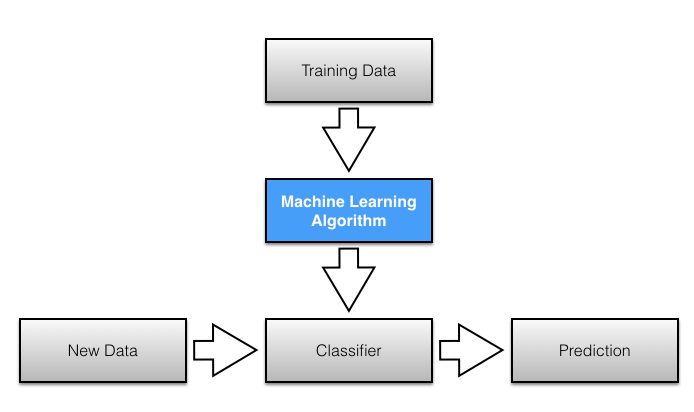
\includegraphics[scale=0.3]{learning_algorithm_basic.png}
\caption{A typical prediction system}
\label{fig:basic_system}
\end{figure}

Before jumping into the algorithms applied, let's talk about the data itself. We have chosen the following 4 categories for our experimentation:
\begin{itemize} 

\item
Backpack (Sample size - 151)
\item
Binoculars (Sample size - 216)
\item
Eiffel Tower (Sample size - 83)
\item
Fried egg (Sample size - 90)

\end{itemize}

Sample of some images from the dataset are shown in Fig.\ref{Fig:sample_dataset}.

\begin{figure}
\centering
\begin{tabular}{|c|c|c|c|}
\hline 
\subfloat{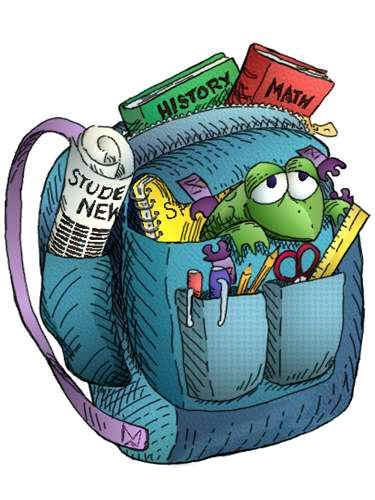
\includegraphics[scale = 0.05]{003_0001.jpg}} &
\subfloat{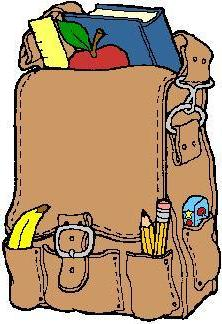
\includegraphics[scale = 0.05]{003_0002.jpg}} &
\subfloat{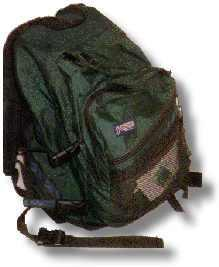
\includegraphics[scale = 0.05]{003_0003.jpg}} &
\subfloat{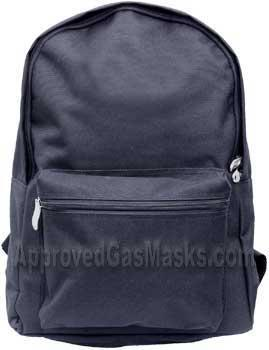
\includegraphics[scale = 0.05]{003_0004.jpg}}\\
\hline
\subfloat{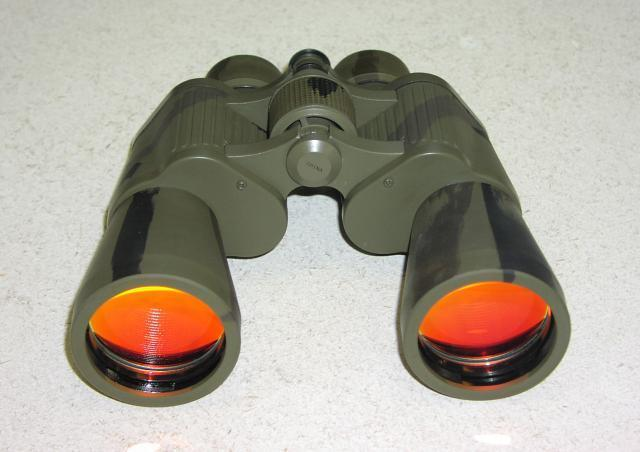
\includegraphics[scale = 0.05]{012_0001.jpg}} &
\subfloat{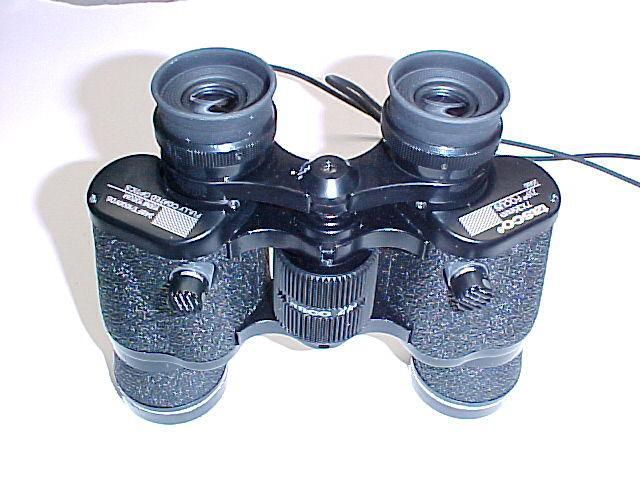
\includegraphics[scale = 0.05]{012_0002.jpg}} &
\subfloat{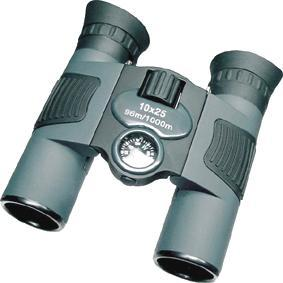
\includegraphics[scale = 0.05]{012_0003.jpg}} &
\subfloat{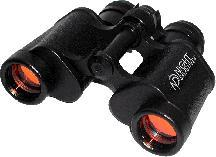
\includegraphics[scale = 0.05]{012_0004.jpg}}\\
\hline 
\subfloat{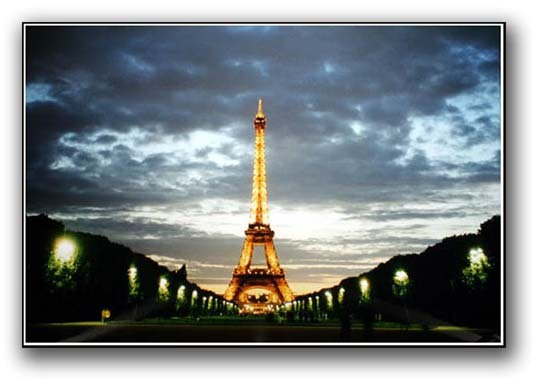
\includegraphics[scale = 0.05]{062_0001.jpg}} &
\subfloat{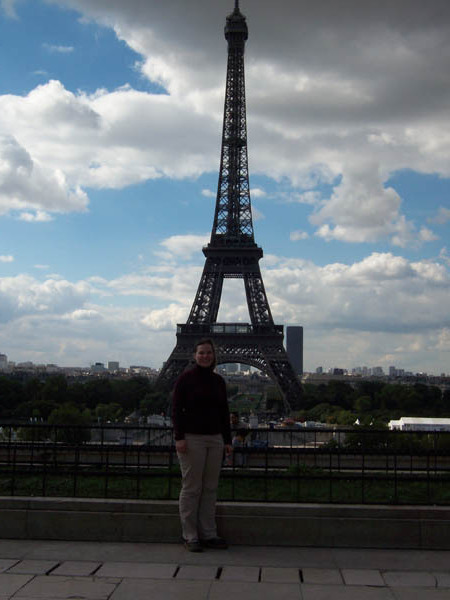
\includegraphics[scale = 0.05]{062_0002.jpg}} &
\subfloat{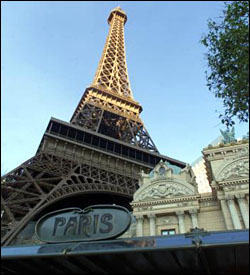
\includegraphics[scale = 0.05]{062_0003.jpg}} &
\subfloat{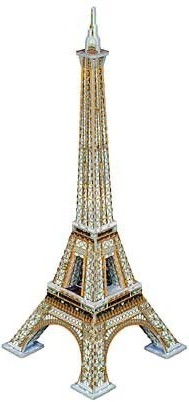
\includegraphics[scale = 0.05]{062_0004.jpg}}\\
\hline 
\subfloat{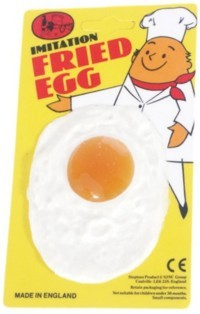
\includegraphics[scale = 0.05]{078_0001.jpg}} &
\subfloat{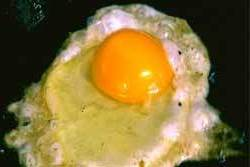
\includegraphics[scale = 0.05]{078_0002.jpg}} &
\subfloat{
\includegraphics[scale = 0.05]{078_0003.jpg}} &
\subfloat{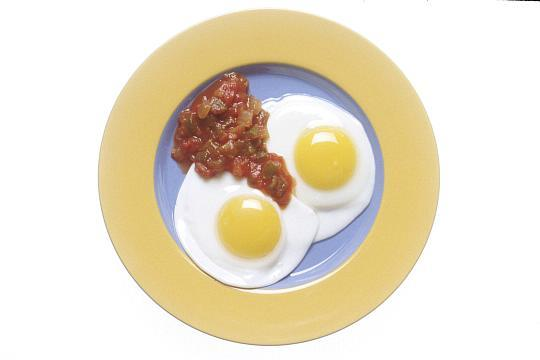
\includegraphics[scale = 0.05]{078_0004.jpg}}\\
\hline

\end{tabular}
\caption{Few samples from our dataset}
\label{Fig:sample_dataset}
\end{figure}

\subsection{Baseline}

For determining baseline, we have used the simple technique of majority class. As seen from above, among the 4 different classes we are experimenting with, binocular has the largest number of sample images. Therefore, given any image from the dataset, the probability of that image having a binocular is highest among the 4 classes. And this is what we use as baseline method.

\subsection{KNN}

Gabor filters are good models of how humans distinguish texture, and are therefore a useful model to use when designing algorithms to recognize texture. This example uses the basic approach described in (A. K. Jain and F. Farrokhnia, "Unsupervised Texture Segmentation Using Gabor Filters",1991) to perform texture segmentation.\cite{Mathworks}

Design an array of Gabor Filters which are tuned to different frequencies and orientations. The set of frequencies and orientations is designed to localize different, roughly orthogonal, subsets of frequency and orientation information in the input image. Regularly sample orientations between [0,150] degrees in steps of 30 degrees. Sample wavelength in increasing powers of two starting from 4/sqrt(2) up to the hypotenuse length of the input image. These combinations of frequency and orientation are taken from [Jain,1991] cited in the introduction.\cite{Mathworks}

Extract gabor magnitude features from source image. When working with Gabor filters, it is common to work with the magnitude response of each filter. Gabor magnitude response is also sometimes referred to as "Gabor Energy". Each MxN Gabor magnitude output image in gabormag(:,:,ind) is the output of the corresponding gabor filter g(ind).\cite{Mathworks}

A nearest-neighbor classification object, where both distance metric ("nearest") and number of neighbors can be altered. The object classifies new observations using the predict method. The object contains the data used for training, so can compute resubstitution predictions.


\subsection{Convolutional Neural Network}
Fully connected neural networks (NN) are not the most suitable architecture to classify images because such a network architecture does not take into account the spatial structure of the images. The spatial location information of individual pixels are lost as soon as we transform it's 2D structure into one dimension to input into the neural network architecture. To solve this problem, LeCunn et. al. came up with convolutional neural network (CNN) in their pioneering work LeNet-5 \cite{LeNet-5_paper}.
\par CNN is a type of feed forward artificial neural network that retains the location information of training data and is well adapted to classify images. The connectivity pattern between it's neurons is inspired by the organization of the animal visual cortex. A typical CNN architecture is shown in Fig.\ref{fig:typical_cnn}.

\begin{figure}[h]
\centering
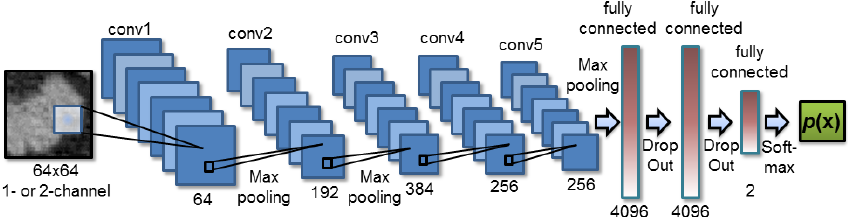
\includegraphics[scale=0.3]{typical_cnn.png}
\caption{A typical CNN architecture}
\label{fig:typical_cnn}
\end{figure}

CNN has 3 components:

\begin{itemize}
\item
Convolutional layer - These layers uses local receptive field and a set of filters to convolve across the width and height of the input volume, computing the dot product between the entries of the filter and the input and producing a 2-dimensional activation map of that filter. As a result, the network learns filters that activate when they see some specific type of feature at some spatial position in the input.
\item
Pooling layer - These layer immediately follow convolutional layer. What the pooling layers do is simplify the information in the output from the convolutional layer. In our experiments we have used max-pooling.
\item
Fully connected layer - These layers are identical to hidden layers of an ANN. They connect the last pooling layer with the output layer. The last layer produces the classification results.
\end{itemize}







\par However, building and training a deep CNN architecture (ConvNet) is not easy because:

\begin{itemize}
\item
There is no exact set of rules which determine how deep or how wide the network should be to produce good accuracy
\item
Small number of data samples per class in Caltech-256 dataset
\item
Huge computational cost of training a ConvNet
\end{itemize}

There are 4 main aspects of ConvNet that we need to determine:

\begin{itemize}
\item
Training data 
	\begin{itemize}
		\item
		How large the training set should be? Should the training set size be increased by augmenting the available images?
		\item
		What should be the resolution of each input image? 
		\item
		What should be the ideal batch size for training the network? 
	\end{itemize}	

\item
Convolutional layers
	\begin{itemize}
		\item
		What should be the depth of the network, i.e., how many convolutional layer should be present?
		\item
		What should be the width of the network, i.e., how many features should be present per convolutional layer?
	\end{itemize}

\item
Fully connected layer
	\begin{itemize}
		\item 
		What should be the depth of the fully connected layer?
		\item
		What should be the size of each fully connected layer, i.e. how many neurons should be present in each fully connected layer?
	\end{itemize}

\item
Prevent overfitting - CNN, like artificial NN can easily overfit. How to prevent that? 
\end{itemize} 

Our focus in this paper is more on trying to understand how tweaking each of the above mentioned aspect affects the performance of ConvNet, rather than to try everything to somehow achieve good accuracy.
\par Since the number of samples per class is quite less, we have increased our training set using image augmentation. We kept 80 images aside for testing. The training set contains 3680 images - 460 are unique images and rest are augmented using rotation of image and adding Gaussian blur.  

We have used dropout, a regularization technique, to prevent overfitting. It is proposed by Hinton et. al. in their seminal paper \cite{dropout_paper}. The term "dropout" refers to dropping out units (both hidden and visible) in a neural network to prevent overfitting.

The networks are created with python and tensorflow. The codebase is available in GitHub \cite{cnn_github}.

\section{Experimental Results}

\subsection{Baseline}

% \centering
\begin{tabular}{|c|c|c|c|c|}
\hline 
&
Backpack &
Binocular &
Eiffel Tower &
Fried Egg \\
\hline 
Backpack &
0 &
20 &
0 &
0 \\
\hline 
Binocular &
0 &
20 &
0 &
0 \\
\hline 
Eiffel Tower &
0 &
20 &
0 &
0 \\
\hline
Fried Egg &
0 &
20 &
0 &
0 \\
\hline
\end{tabular}


\subsection{KNN}

% \centering
\begin{tabular}{|c|c|c|c|c|}
\hline 
&
Backpack &
Binocular &
Eiffel Tower &
Fried Egg \\
\hline 
Backpack &
12 &
5 &
0 &
3 \\
\hline 
Binocular &
3 &
17 &
0 &
0 \\
\hline 
Eiffel Tower &
3 &
5 &
9 &
3 \\
\hline
Fried Egg &
3 &
8 &
1 &
8 \\
\hline
\end{tabular}


\subsection{Convolutional Neural Network}


\begin{table}[htbp]
    \begin{center}
    \begin{tabularx}{1.2\textwidth}{|c|X|X|X|X|X|X|X|X|}
        \hline
        Index & Input image size & Conv layer 1 & Conv layer 2 & Conv layer 3 & Fully connected layer 1 & Fully connected layer 2 & Train accuracy & Test accuracy \\
        \hline 
        CNN 1 & 28x28x1 & 14x14x32 & 7x7x64 & NA & 64x1 & NA & 45.43\% & 26.25\% \\
        \hline
        CNN 2 & 28x28x1 & 14x14x32 & 7x7x64 & NA & 1024x1 & NA & 79.78\% & 27.50\% \\
        \hline
        CNN 3 & 64x64x1 & 32x32x32 & 16x16x64 & 8x8x128 & 1024x1 & NA & 91.00\% & 42.50\% \\
        \hline
        CNN 4 & 28x28x1 & 14x14x64 & 7x7x128 & NA & 1024x1 & 1024x1 & 96.82\% & 69.69\% \\
        \hline
        CNN 5 & 28x28x1 & 14x14x128 & 7x7x256 & NA & 1024x1 & 1024x1 & 96.54\% & 67.81\% \\
        \hline
    \end{tabularx}
    \caption{Results of 5 different CNN architectures}
    \end{center}
\end{table}

\underline{Some interesting observations from the result above are:}
\begin{itemize}
\item
A very shallow network cannot capture enough information about the different categories of images to provide good testing accuracy (CNN 1 and CNN 2)
\item
Increasing the depth of convolution layer results better testing accuracy (CNN 3). This can be attributed to the fact that more complicated features are captured by the convolutional layers, which describes the objects more accurately
\item
Increasing depth of fully connected layers, even with less convolutional layers, boosts accuracy by a large percentage (CNN 4). We believe this is because more hidden layers learn hierarchical representations of the input data and can better generalize to unseen data as well
\item
We do not achieve better accuracy by just making the network wide and not deep (CNN 5). The reason, we believe, is even though there are more features, they are not much different from the existing ones to help distinguish the categories any better than CNN 4
\end{itemize}


\section{Conclusion}

The project was an exploration across various approaches to object recognition across time. We started with simpler model like KNN and moved to extremely complex models like CNN and everything in between. Fig.\ref{fig:results_comparison} shows the comparison of the various experimental results we captured in this project.

\begin{figure}[h]
\centering
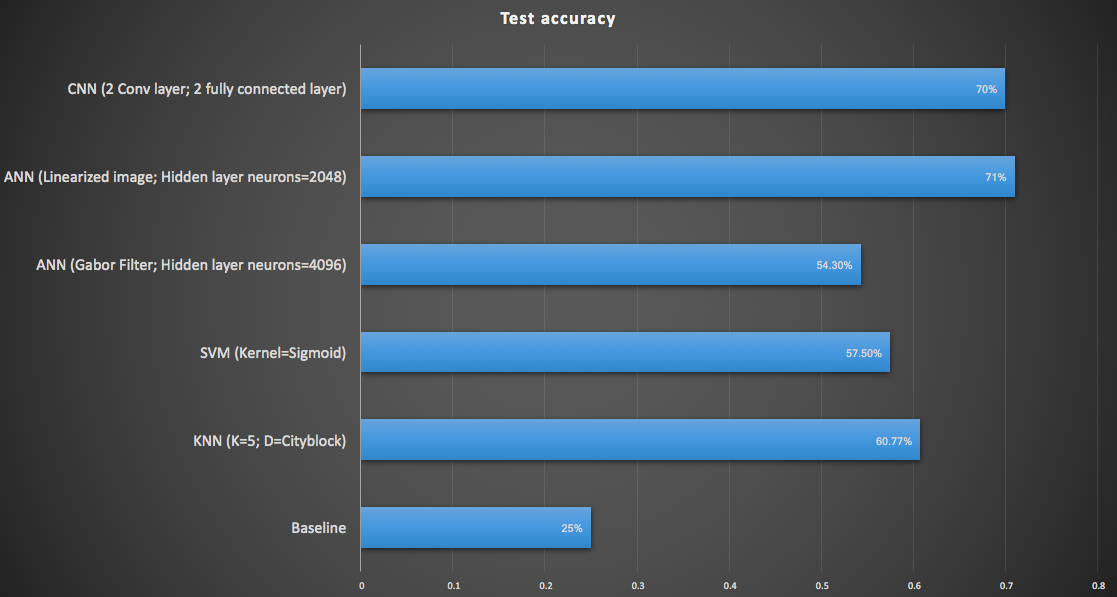
\includegraphics[scale=0.3]{results_comparison2.png}
\caption{A comparison of experimental results}
\label{fig:results_comparison}
\end{figure}

\underline{The comparison of the results yield some very interesting points:}
\begin{itemize}
\item
Neural networks trained with the raw image itself (i.e. without any feature engineering) produces much better results in terms of accuracy than algorithms with feature engineering.
\item
Feature engineering for large categories of object is fragile. There are lot of parameters that need to be decided to get good accuracy and there is no guarantee that introduction of a new category won't degrade the performance.
\item
One of the best advantage of deep convolutional neural network is the independence from feature engineering. This makes the approach more robust.
\end{itemize}

\underline{The take home point, for us, from doing this project are:}
\begin{itemize}
\item
Handcrafted features for large variety of images is unreliable and fragile
\item
Featureless approach to computer vision problem with deep neural network yields better accuracy
\item
Modern computer vision research is moving towards featureless approach with deep ConvNet. 
Ex: ImageNet and GoogLeNet
\end{itemize}

% In fact, during our research for different approaches for object recognition taken across time, we noticed the shift from complicated feature engineering based approach to a deep network based approach. Histogram of Gradients (HoG), SIFT, SURF and BRISK are some of the most complicated and powerful feature descriptors present and yet ImageNet and GoogLeNet have beat them significantly. These deep networks are used widely in search engines and voice recognition and they perform quite well in a robust manner. 


\begin{thebibliography}{9}

\bibitem{caltech_dataset_paper} 
Greg Griffin, Alex Holub and Pietro Perona. \\
\textit{Caltech-256 Object Category Dataset}. 
 
\bibitem{knn_svm_paper} 
Hao Zhang, Alexander C. Berg, Michael Maire and Jitendra Malik \\
\textit{SVM-KNN: Discriminative Nearest Neighbor Classification for Visual Category
Recognition}.
 
\bibitem{knuthwebsite} 
Knuth: Computers and Typesetting,
\\\texttt{http://www-cs-faculty.stanford.edu/\~{}uno/abcde.html}

\bibitem{Mathworks} 
Texture Segmentation using Gabor Filters
\\\texttt{https://www.mathworks.com/help/images/texture-segmentation-using-gabor-filters.html}

\bibitem{Gabor_Paper} 
Simona E.Grigorescu, Nicolai Petkov, and Peter Kruizinga\\\
\textit{Comparison of Texture Features based on Gabor Filters}. 

\bibitem{Gabor_Paper_Jain} 
Anil K. Jain,Farshid Farrokhnia
\\
\textit{Unsupervised Texture Segmentation Using Gabor
Filters}. 

\bibitem{LeNet-5_paper}
Yann Lecun, Leon Bottou, Yoshua Bengio and Patrick Haffner \\
\textit{Gradient-Based learning applied to document recognition}

\bibitem{dropout_paper}
Nitish Srivastava,
Geoffrey Hinton,
Alex Krizhevsky,
Ilya Sutskever and
Ruslan Salakhutdinov 
\textit{Dropout: A Simple Way to Prevent Neural Networks from Overfitting}

\bibitem{cnn_github}
\textit{https://github.com/anubhabMajumdar/Object-Recognition-using-ConvNet}

\end{thebibliography}

\end{document}
